\documentclass[conference]{IEEEtran}
\IEEEoverridecommandlockouts
\usepackage{booktabs,graphicx,amsmath,cite}
\usepackage[hidelinks]{hyperref}

\title{Interpreting Credit-Risk Decisions Through a Diverse Counterfactual Explanation Framework}
\author{\IEEEauthorblockN{Anonymous Author(s)}
\IEEEauthorblockA{Affiliation withheld for review}}

\begin{document}
\maketitle

\begin{abstract}
Machine-learning credit-risk models support scalable assessment, but an adverse prediction alone offers little guidance about what would need to differ for the same model to produce a favorable outcome. This paper examines whether diverse counterfactual explanations remain available and interpretable when the predictive model is changed. Five classifier families---class-weighted logistic regression, decision tree, random forest, AdaBoost, and XGBoost---are trained on the German Credit, Give Me Some Credit, and Taiwan Credit datasets using identical stratified splits and preprocessing. For the ten test cases assigned the highest default probabilities by each classifier, the model-agnostic genetic-search implementation of Diverse Counterfactual Explanations (DiCE) requests four alternative profiles that reduce predicted default probability below 0.50. The search preserves designated immutable attributes and imposes dataset-specific directional restrictions. XGBoost achieved the highest ROC--AUC on all datasets (0.809, 0.869, and 0.777), while the decision tree achieved the lowest (0.649, 0.688, and 0.673). Counterfactual coverage was 100\% in 13 of 15 model--dataset settings; logistic regression reached only 50\% on Give Me Some Credit, and AdaBoost reached 90\% on German Credit. The decision tree generally returned the sparsest explanations, but this simplicity coincided with weaker predictive discrimination. Taiwan Credit required substantially more simultaneous changes for every classifier. The results show that predictive performance and counterfactual recourse quality are distinct: conclusions obtained from one classifier may not generalize to another. These counterfactuals characterize model decision boundaries rather than causal interventions and require domain validation before use in lending.
\end{abstract}

\begin{IEEEkeywords}
credit scoring, counterfactual explanations, explainable artificial intelligence, algorithmic recourse, DiCE
\end{IEEEkeywords}

\section{Introduction}
Machine-learning models are increasingly studied for credit scoring because they can extract predictive structure from heterogeneous applicant and repayment data. Their use in a high-impact domain nevertheless raises a practical interpretability problem. A probability of default communicates a model assessment, but it does not identify what would need to differ for the model to reach another outcome. Feature importance is insufficient for this purpose: an influential variable may be immutable, infeasible to change, or incapable of reversing a prediction by itself.

Counterfactual explanations address this gap by constructing alternative profiles that receive a desired model output. Rather than stating only that repayment history was influential, a counterfactual may specify a combination of lower utilization, fewer delinquencies, or different loan terms that moves a classifier below its adverse threshold. This form of explanation is local, contrastive, and linked directly to a decision \cite{wachter2018counterfactual,ustun2019recourse}. Useful explanations should, however, be valid, close to the original case, sparse, plausible, diverse, and restricted to attributes that may legitimately vary \cite{mothilal2020dice,verma2020review}.

The predictive model is itself an important source of variation. Linear, piecewise-constant, bagged, and boosted boundaries can assign different risks to the same population and require different changes to cross a common threshold. A study based on one classifier may therefore conflate properties of the explanation algorithm with properties of the underlying model.

This paper asks: \emph{How does predictive model choice affect the availability and characteristics of genetically optimized counterfactual explanations in credit-risk classification?} We hold the explanation framework constant and compare five classifier families across three benchmark datasets. Our contributions are: (1) a controlled multi-model genetic-DiCE evaluation using common preprocessing and constraints; (2) joint reporting of predictive performance, validity, coverage, sparsity, proximity, and diversity; and (3) evidence that predictive discrimination and access to concise recourse do not necessarily align.

\section{Related Work}
Wachter, Mittelstadt, and Russell described counterfactual explanations as nearby cases that obtain a different automated outcome without disclosing a model's internal logic \cite{wachter2018counterfactual}. Algorithmic-recourse research similarly emphasizes a person's ability to obtain a desired classification by altering actionable inputs. Ustun, Spangher, and Liu demonstrated that standard modeling choices can materially affect recourse in linear classification \cite{ustun2019recourse}.

Mothilal, Sharma, and Tan proposed Diverse Counterfactual Explanations (DiCE), which generates sets of alternatives rather than one solution \cite{mothilal2020dice}. Its formulation balances outcome validity and proximity while encouraging diversity. Multiple alternatives matter because decision subjects may face different practical constraints. Reviews distinguish validity, proximity, sparsity, plausibility, diversity, actionability, causality, and fairness as separate dimensions of counterfactual quality \cite{verma2020review}.

Credit scoring is a natural but difficult recourse setting. Applicant records combine immutable demographics, potentially actionable financial conditions, and historical variables that cannot literally be rewritten. Correlated monthly measures may also yield mathematically valid but operationally implausible profiles. This study therefore treats DiCE outputs as explanations of fitted classifiers, not causal prescriptions.

\section{Methodology}
\subsection{Data and Preprocessing}
Three public benchmarks are used. German Credit contains 1,000 applicants and credit, savings, employment, housing, and personal attributes. Give Me Some Credit contains 150,000 records with utilization, income, debt, credit-line, dependent, age, and delinquency variables. Taiwan Credit contains 30,000 records with credit limits, demographics, monthly bills, payments, repayment status, and subsequent default. The binary outcome equals one for default.

Each dataset is divided into stratified 75\% training and 25\% test partitions with random seed 42. Numeric features are median-imputed and standardized. Categorical features are mode-imputed and one-hot encoded. The held-out samples contain 250, 37,500, and 7,500 observations, with default rates of 0.300, 0.067, and 0.221, respectively.

\subsection{Predictive Models}
Five classifiers are trained separately: class-weighted logistic regression; a balanced decision tree with minimum leaf size five; a 300-tree balanced random forest with minimum leaf size two; AdaBoost with 200 estimators, learning rate 0.5, and balanced sample weights; and XGBoost with 300 estimators, maximum depth four, learning rate 0.05, row and feature subsampling of 0.8, and class-ratio weighting. Predicted probabilities at or above 0.50 are assigned to default. Evaluation includes ROC--AUC, average precision, accuracy, balanced accuracy, F1, and Brier score.

\subsection{Genetic DiCE}
Let $f(x)$ be the estimated default probability for profile $x$. A counterfactual $x'$ is valid when
\begin{equation} f(x') < 0.50. \end{equation}
For each model--dataset pair, the ten test cases with the largest predicted default probabilities form a high-risk stress-test cohort. DiCE's model-agnostic genetic search requests four class-0 alternatives per query. Proximity, diversity, and sparsity weights are 1.0, 1.0, and 0.5; post-hoc sparsity is 0.1. The objective balances prediction loss, distance, and sparsity while rewarding diversity among alternatives \cite{mothilal2020dice}.

Dataset-specific policies fix immutable attributes. German Credit fixes age, personal-status/sex, and foreign-worker status; duration, credit amount, and installment rate may only decrease. Give Me Some Credit fixes age; income may increase, while utilization, debt ratio, and delinquencies may decrease. Taiwan fixes sex, education, marital status, and age; credit limit and payment amounts may increase, while delay indicators may decrease.

Validity is independently recalculated from returned profiles. Coverage is the fraction of queries receiving at least one valid result. Sparsity is the number of original features changed. Proximity uses IQR-normalized numeric differences and unit categorical mismatch penalties:
\begin{equation}
d(x,x')=\frac{1}{p}\left[\sum_{j\in N}\frac{|x_j-x'_j|}{\mathrm{IQR}(X_j)}+\sum_{j\in C}\mathbf{1}(x_j\neq x'_j)\right].
\end{equation}
Diversity is the mean pairwise mixed-type distance within a returned set. Raw distances are interpreted within datasets because feature spaces differ.

\section{Results}
\subsection{Predictive Performance}
Table~\ref{tab:auc} reports ROC--AUC. XGBoost ranked first on all datasets, while the single tree ranked last. Accuracy alone was misleading under imbalance: on Give Me Some Credit, random forest accuracy was 0.934 but balanced accuracy was 0.638, whereas XGBoost achieved 0.799 and 0.787, respectively.

\begin{table}[t]
\caption{Held-Out ROC--AUC}
\label{tab:auc}
\centering\small
\begin{tabular}{lccc}
\toprule Model & German & GMSC & Taiwan \\
\midrule
Logistic regression & 0.807 & 0.800 & 0.716 \\
Decision tree & 0.649 & 0.688 & 0.673 \\
Random forest & 0.797 & 0.851 & 0.768 \\
AdaBoost & 0.794 & 0.861 & 0.768 \\
XGBoost & \textbf{0.809} & \textbf{0.869} & \textbf{0.777} \\
\bottomrule
\end{tabular}
\end{table}

\subsection{Counterfactual Performance}
Table~\ref{tab:cf} summarizes genetic DiCE. Thirteen of 15 settings achieved full coverage. Logistic regression covered only five of ten Give Me Some Credit cases; AdaBoost missed one German query. Most generated profiles were valid, although decision-tree and XGBoost validity on Give Me Some Credit were 92.5\% and 95.0\%.

\begin{table*}[t]
\caption{Genetic DiCE Results for Ten High-Risk Queries per Cell}
\label{tab:cf}
\centering\small
\begin{tabular}{llrrrr}
\toprule Dataset & Model & Generated & Validity (\%) & Coverage (\%) & Mean changes \\
\midrule
German & Logistic & 35 & 100.0 & 100 & 4.29 \\
 & Tree & 40 & 100.0 & 100 & \textbf{2.70} \\
 & Forest & 32 & 100.0 & 100 & 3.03 \\
 & AdaBoost & 31 & 100.0 & 90 & 3.29 \\
 & XGBoost & 35 & 100.0 & 100 & 3.26 \\
\midrule
GMSC & Logistic & 17 & 100.0 & 50 & 5.12 \\
 & Tree & 40 & 92.5 & 100 & \textbf{4.00} \\
 & Forest & 39 & 100.0 & 100 & 4.56 \\
 & AdaBoost & 40 & 100.0 & 100 & 6.45 \\
 & XGBoost & 40 & 95.0 & 100 & 5.29 \\
\midrule
Taiwan & Logistic & 37 & 100.0 & 100 & 13.46 \\
 & Tree & 39 & 100.0 & 100 & \textbf{10.18} \\
 & Forest & 38 & 100.0 & 100 & 12.45 \\
 & AdaBoost & 29 & 100.0 & 100 & 14.52 \\
 & XGBoost & 38 & 100.0 & 100 & 13.84 \\
\bottomrule
\end{tabular}
\end{table*}

The decision tree produced the sparsest explanations across all datasets, but also the weakest discrimination. Taiwan required many more changes under every classifier, reflecting coordinated alterations across monthly repayment, billing, and payment variables. Thus, representational complexity translated into larger counterfactual burden.

\begin{figure*}[t]
\centering
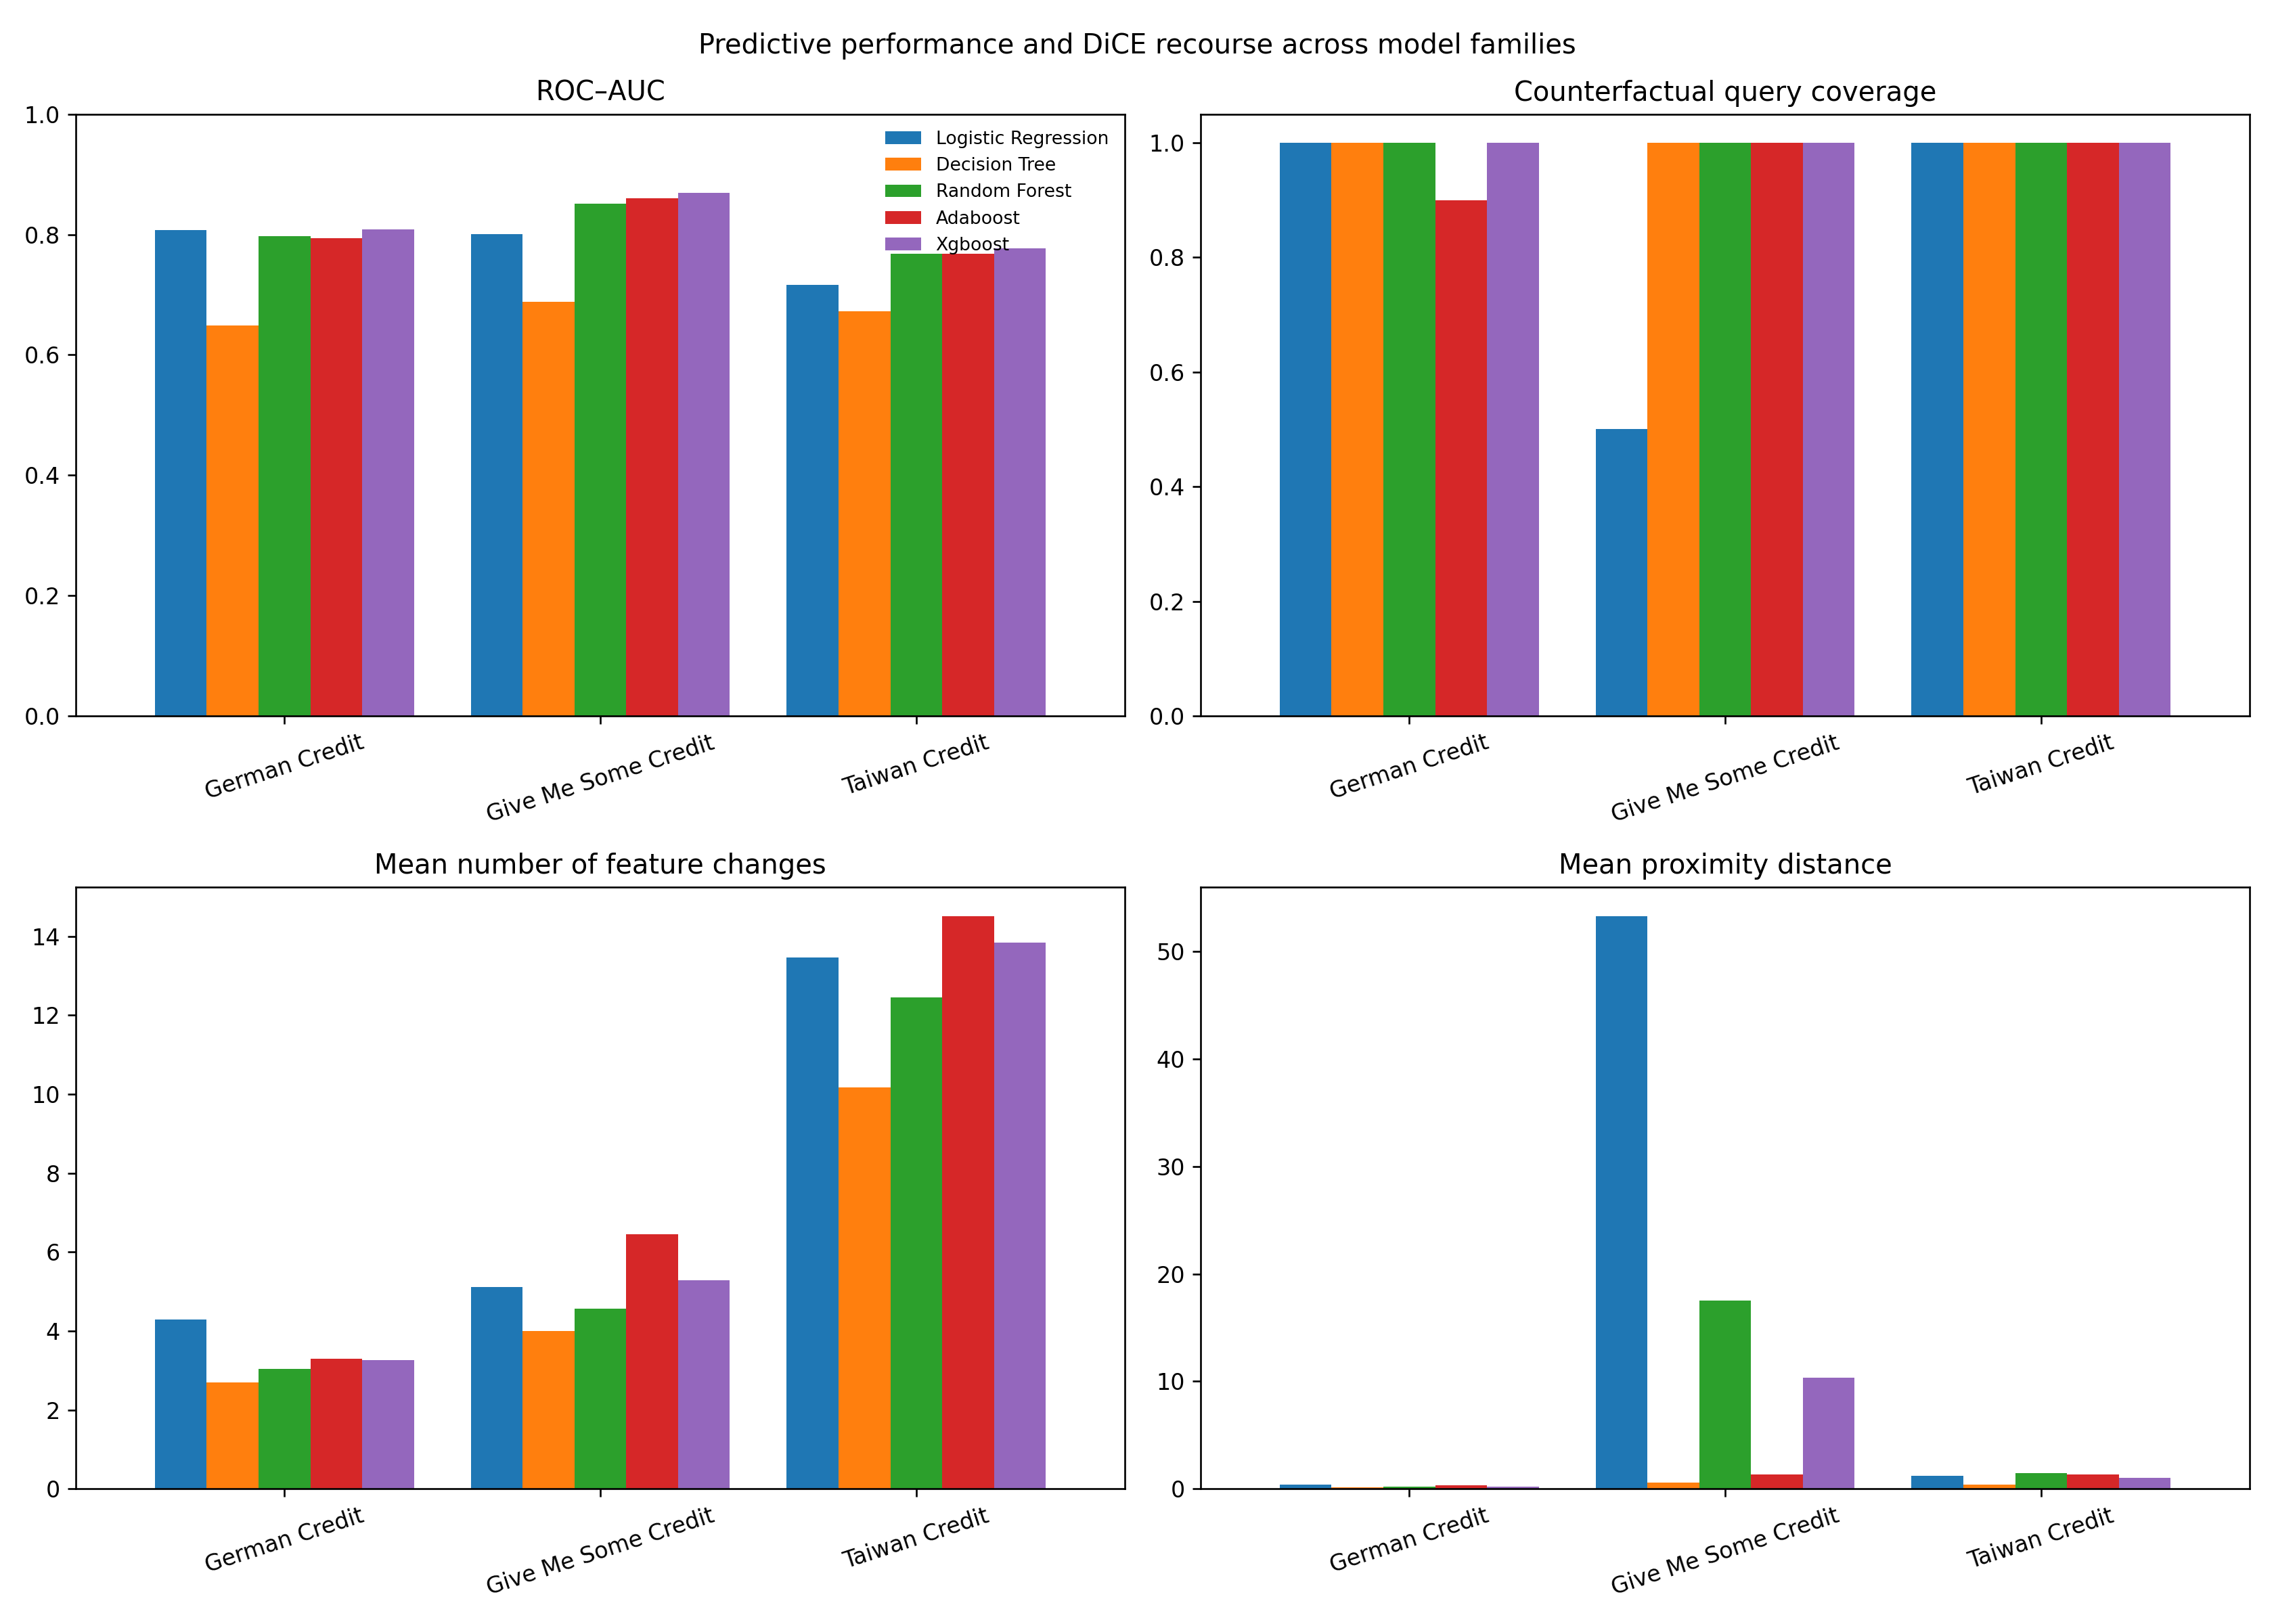
\includegraphics[width=.96\textwidth]{../figures/model_comparison.png}
\caption{Predictive performance and genetic-DiCE recourse across model families.}
\label{fig:comparison}
\end{figure*}

German counterfactuals were relatively close under all models. Give Me Some Credit yielded extreme distances for some models: mean logistic proximity was 53.32 and random-forest proximity 17.50. The data contain special delinquency values such as 96 and 98; treating them as ordinary counts can dominate normalized distance and create extreme scores. These magnitudes are therefore evidence of data-representation sensitivity, not intrinsically better diversity.

\section{Discussion}
The results demonstrate that counterfactual explanations are conditional on the model being explained. Holding the generator, threshold, and constraints constant did not eliminate differences in coverage or burden. A single-model study may consequently mistake decision geometry for a general property of credit recourse.

No classifier dominated both prediction and explanation. XGBoost offered the strongest ROC--AUC, whereas the decision tree offered the fewest changes. The latter simplicity should not be interpreted as superiority because it coincided with materially weaker prediction. Coverage also matters: explanations that are excellent for easy cases but unavailable to extreme-risk cases cannot provide universal recourse.

Validity alone remains insufficient. A classifier changes output when supplied a returned profile, but the profile may be distant, historically impossible, or unavailable to an applicant. These explanations are algorithmic rather than causal: they do not show that enacting a change would reduce real default risk.

\section{Limitations}
The study is a ten-case-per-model stress test, not a population estimate. Each model selects its own highest-risk cases, preventing paired applicant-level inference. Repeated seeds are required to quantify genetic-search stability. Constraints do not fully encode temporal or institutional feasibility. Special delinquency codes require cleaning and sensitivity analysis. Distances are not directly comparable across heterogeneous datasets. Freezing protected attributes is not a fairness analysis, and subgroup disparities in coverage and cost remain untested. Finally, the datasets contain default outcomes rather than historical lender decisions; ``adverse'' denotes predicted default, not observed denial.

\section{Conclusion and Future Work}
Across five classifiers and three credit datasets, model choice materially altered genetic-DiCE coverage and explanation complexity. XGBoost achieved the best predictive discrimination, while a single tree produced the sparsest explanations at a predictive cost. Logistic regression failed to provide recourse for half of the most extreme Give Me Some Credit cases, and Taiwan required many simultaneous changes regardless of model.

Future work will evaluate a larger shared query cohort, repeat search across seeds, report confidence intervals and paired tests, clean anomalous codes, distinguish strict applicant recourse from permissive model auditing, and assess subgroup disparities. These steps are necessary before counterfactual explanations can be treated as equitable guidance rather than descriptions of a model boundary.

\bibliographystyle{IEEEtran}
\bibliography{references}
\end{document}
